\documentclass[a4paper]{article}
\usepackage{ctex}
\usepackage[affil-it]{authblk}
\usepackage{float}
\usepackage{amsmath, amssymb, amsthm, amsfonts}
% \usepackage[backend=bibtex,style=numeric]{biblatex}
\usepackage{graphicx}
\usepackage{hyperref}
\usepackage{physics}
% 设置超链接样式
\hypersetup{
	colorlinks=true,
	linkcolor=blue,
	citecolor=blue,
	urlcolor=blue,
}

\usepackage{listings}
\usepackage{color}

\definecolor{mygray}{rgb}{0.4,0.4,0.4}
\definecolor{mygreen}{rgb}{0,0.8,0.6}
\definecolor{myorange}{rgb}{1.0,0.4,0}

\lstset{
	basicstyle=\footnotesize\sffamily\color{black},
	breaklines=true,
	commentstyle=\color{mygray},
	frame=single,
	numbers=left,
	numbersep=5pt,
	numberstyle=\tiny\color{mygray},
	keywordstyle=\color{mygreen},
	showspaces=false,
	showstringspaces=false,
	stringstyle=\color{myorange},
	tabsize=2
}

\usepackage{geometry}
\geometry{margin=1.5cm, vmargin={0pt,1cm}}
\setlength{\topmargin}{-1cm}
\setlength{\paperheight}{29.7cm}
\setlength{\textheight}{25.3cm}

\usepackage[titletoc,title]{appendix}
\usepackage{subcaption}
% \usepackage{subfigure}


\begin{document}
% =================================================
\title{Numerical Analysis Project}

\author{王昊 Wang Hao 3220104819}

\maketitle

\tableofcontents
\newpage

\section{A. Cubic Interpolation Of $\frac{1}{1+25x^2}$}
I use the periodic condition to interpolate the function $\frac{1}{1+25x^2}$ on the interval $[-1,1]$.

And here is the result:
\begin{figure}[H]
    \centering
    \begin{subfigure}[b]{0.4\textwidth}
        \centering
        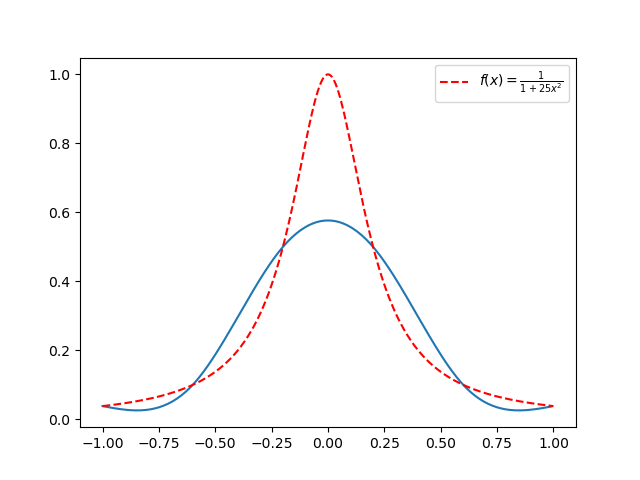
\includegraphics[width=\textwidth]{../figure/A_6.png}
        \caption{$N=6$}
    \end{subfigure}
    \begin{subfigure}[b]{0.4\textwidth}
        \centering
        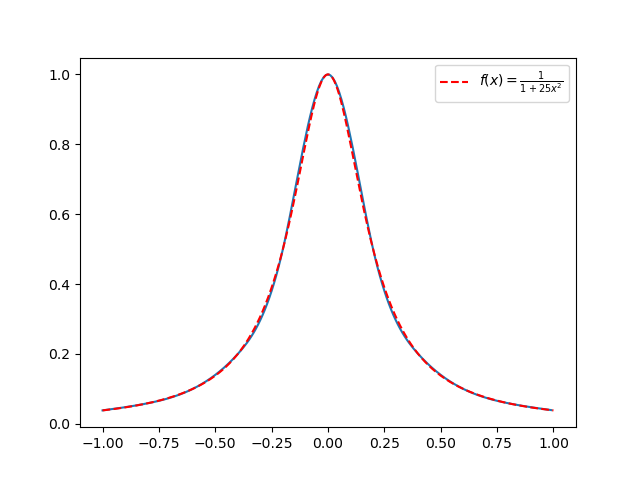
\includegraphics[width=\textwidth]{../figure/A_11.png}
        \caption{$N=11$}
    \end{subfigure}
    \\
    \begin{subfigure}[b]{0.4\textwidth}
        \centering
        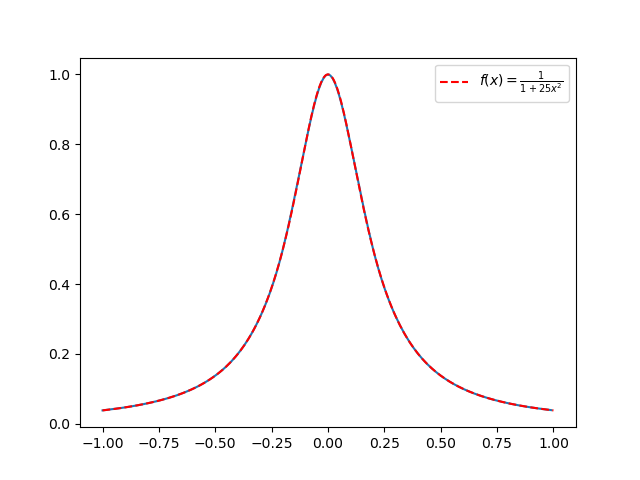
\includegraphics[width=\textwidth]{../figure/A_21.png}
        \caption{$N=21$}
    \end{subfigure}
    \begin{subfigure}[b]{0.4\textwidth}
        \centering
        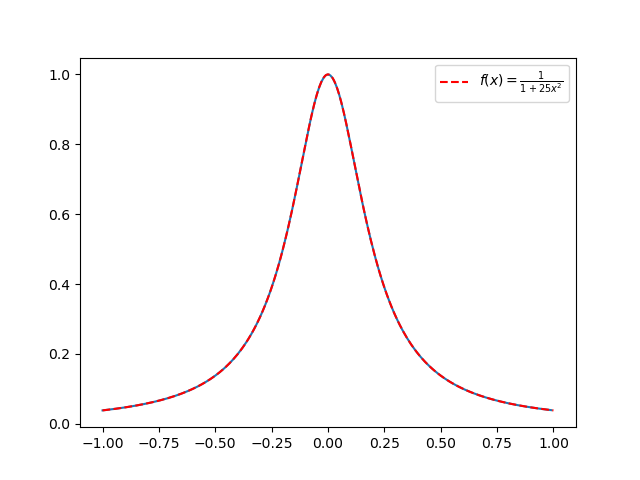
\includegraphics[width=\textwidth]{../figure/A_41.png}
        \caption{$N=41$}
    \end{subfigure}
    \\
    \begin{subfigure}[b]{0.4\textwidth}
        \centering
        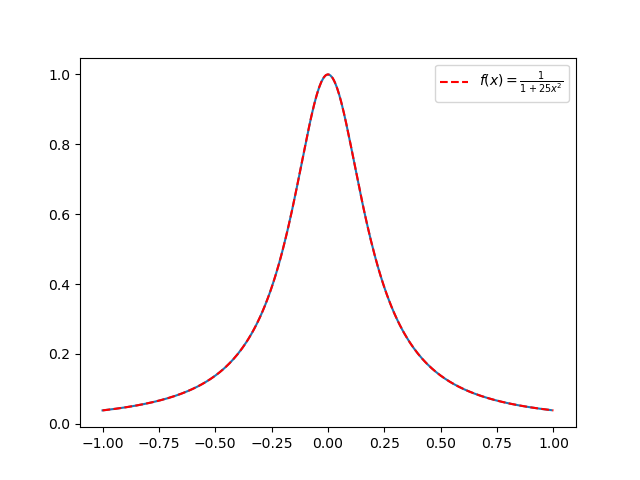
\includegraphics[width=\textwidth]{../figure/A_81.png}
        \caption{$N=81$}
    \end{subfigure}
\end{figure}

For the maximum error, we have the following table:
\begin{table}[H]
    \centering
    \begin{tabular}{|c|c|}
        \hline
        $N$ & Max Error \\
        \hline
        6 & 0.423482 \\
        11 & 0.0205306 \\
        21 & 0.00316894 \\
        41 & 0.000275356 \\
        81 & 1.609e-05 \\
        \hline
    \end{tabular}
\end{table}

Assuming that the error is $y = A N^n$, we have $\log\qty(y) = \log\qty(A) + n \log\qty(N)$. 

By LeastSquares, we have $n \approx -3.78032$, which means cubic spline has 4th order convergence.

\section{C. Spline for $f(x) = \frac{1}{1 + x^5}$}

For Thm3.57, we have the following result figure
\begin{figure}[H]
    \centering
    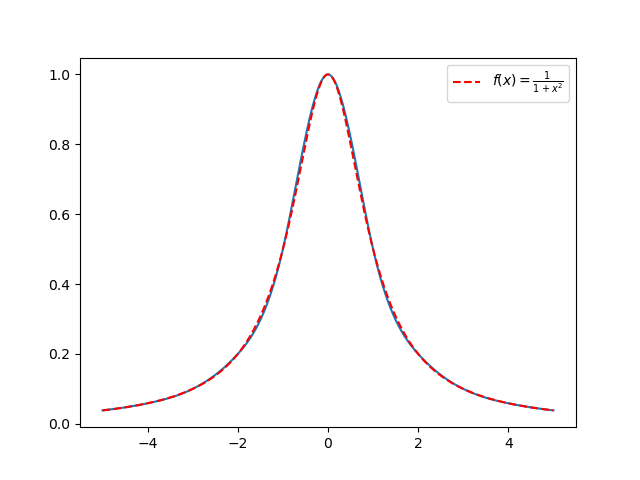
\includegraphics[width=0.5\textwidth]{../figure/C_3.png}
    \caption{$N=3$}
\end{figure}

For Thm3.58, we have the following result figure
\begin{figure}[H]
    \centering
    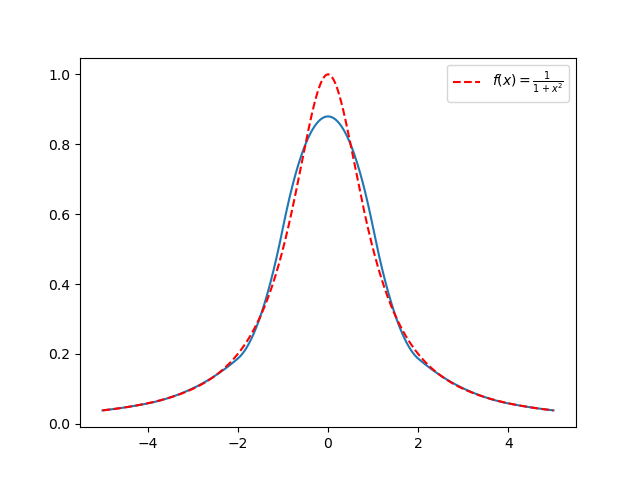
\includegraphics[width=0.5\textwidth]{../figure/C_2.png}
    \caption{$N=2$}
\end{figure}
This result is not so good, because $t_i = -\frac{11}{2} + i$ doesn't have $0$ in them.

\section{D. Error of The Two Cardinal Splines}

For the errors at the points
\begin{equation}
    x = -3.5, -2.5, -1.5, -0.5, 0, 0.5, 1.5, 2.5, 3.5.
\end{equation}
We can also draw a table
\begin{table}[H]
    \centering
    \begin{tabular}{|c|c|c|}
        \hline
        $x$ & N=3 & N=2 \\
        \hline
        -3.5 & 0.000669568 & 0 \\
        -2.5 & 0.00211777 & 2.77556e-17 \\
        -1.5 & 0.0103367 & 0 \\
        -0.5 & 0.0205289 & 1.11022e-16 \\
        0 & 0 & 0.120238 \\
        0.5 & 0.0205289 & 1.11022e-16 \\
        1.5 & 0.0103367 & 0 \\
        2.5 & 0.00211777 & 0 \\
        3.5 & 0.000669568 & 0 \\
        \hline
    \end{tabular}
\end{table}

For the Quadratic Cardinal Spline, because these points are its knots, so the error is small enough, 
some are close to machine precision because that the solver is not exact and we have floating point error.

The Cubic Spline is better, its max error is smaller than the Quadratic Cardinal Spline.


\section{E. Curve Fitting}

\subsection{I. Fit Heart Curve by Cumulative chordal length}

The Heart Curve is defined as
\begin{equation}
    x^2 + (\frac{3}{2} y + \sqrt{\abs{x}})^2 = 3.
\end{equation}
Then we can have 
\begin{equation}
    x = \sqrt{3} \sin t, \\ 
    y = \frac{2}{3} (\sqrt{3} \cos t + \sqrt{\sqrt{3} |\sin t|})
\end{equation}

Then, use the \textbf{Periodic Condition} we can have 
\begin{figure}[H]
    \centering
    \begin{subfigure}[b]{0.35\textwidth}
        \centering
        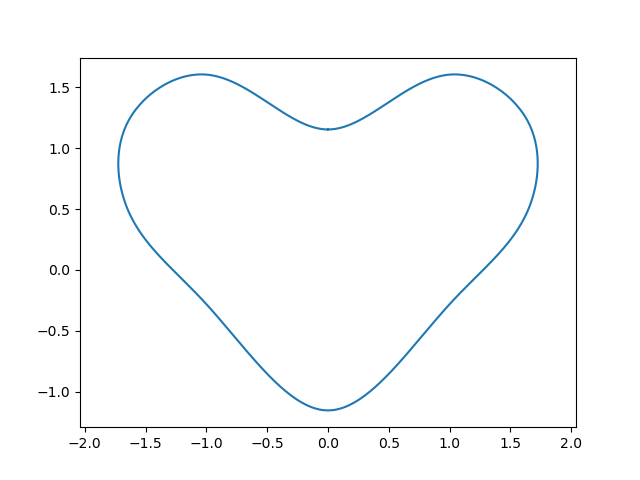
\includegraphics[width=\textwidth]{../figure/E_heart_cum_PP10.png}
        \caption{$N = 10$}
    \end{subfigure}
    \begin{subfigure}[b]{0.35\textwidth}
        \centering
        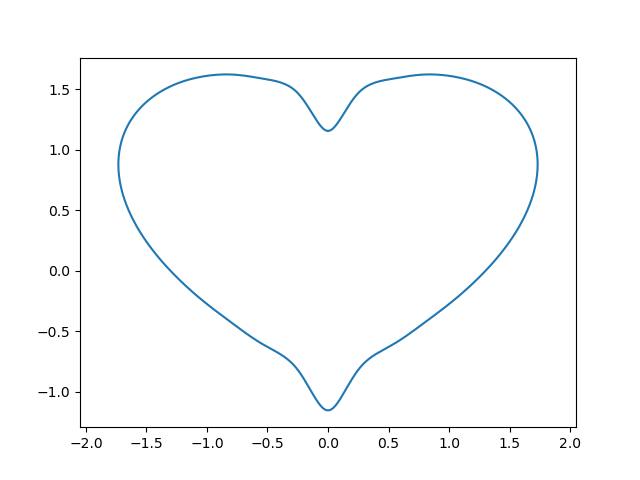
\includegraphics[width=\textwidth]{../figure/E_heart_cum_PP40.png}
        \caption{$N = 40$}
    \end{subfigure}
    \\ 
    \begin{subfigure}[b]{0.35\textwidth}
        \centering
        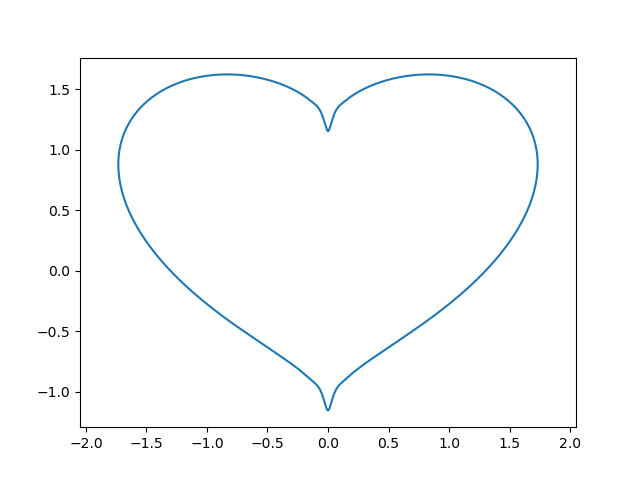
\includegraphics[width=\textwidth]{../figure/E_heart_cum_PP160.png}
        \caption{$N = 160$}
    \end{subfigure}
\end{figure}

For the \textbf{Evenly Spaced} knots, we can also draw similiar pictures
\begin{figure}[H]
    \centering
    \begin{subfigure}[b]{0.35\textwidth}
        \centering
        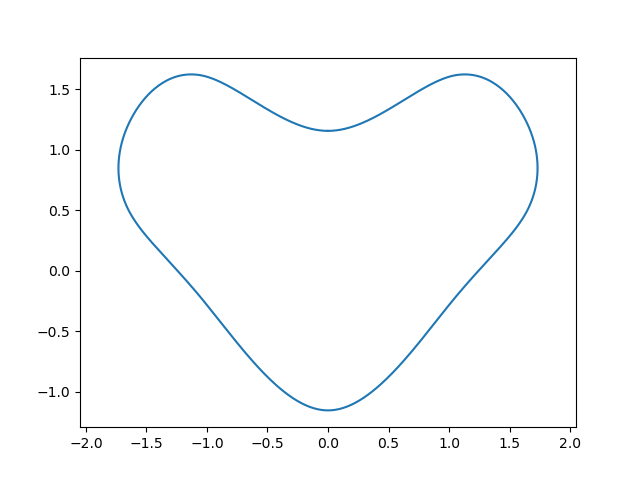
\includegraphics[width=\textwidth]{../figure/E_heart_PP10.png}
        \caption{$N = 10$}
    \end{subfigure}
    \begin{subfigure}[b]{0.35\textwidth}
        \centering
        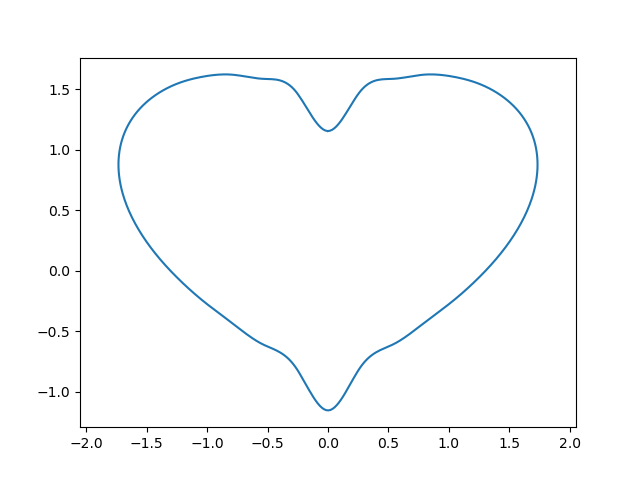
\includegraphics[width=\textwidth]{../figure/E_heart_PP40.png}
        \caption{$N = 40$}
    \end{subfigure}
    \\ 
    \begin{subfigure}[b]{0.35\textwidth}
        \centering
        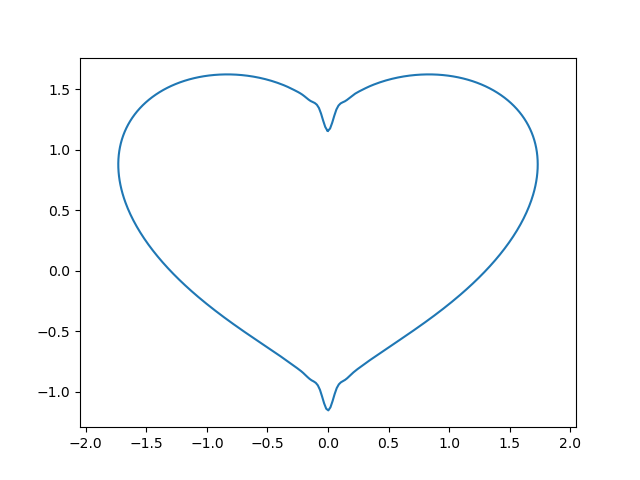
\includegraphics[width=\textwidth]{../figure/E_heart_PP160.png}
        \caption{$N = 160$}
    \end{subfigure}
\end{figure}

Surely the Cumulative chordal length is better than the evenly spaced knots.




\subsection{II. Fit Two Dimension Curve}
Here we fit the curve 
\begin{equation}
    x = \sin t + t \cos t, \\
    y = \cos t - t \sin t.
\end{equation}
In the interval $[0, 6\pi]$ is absolutely not periodic, so we use the \textbf{Complete Spline} to fit it. 

We can have the following result 
\begin{equation}
    x^{\prime}(0) = 2.0, x^{\prime}(6 \pi) = 2.0, \\
    y^{\prime}(0) = 0.0, y^{\prime}(6 \pi) = -6 \pi. 
\end{equation}

For the cumulative chordal length, we can approximate the derivate by arc length, 
$\mathrm{d} s = \sqrt{4+t^2} \mathrm{d} t$, so we can have similiar result 
\begin{equation}
    x^{\prime}(0) = 2.0 / \sqrt{4}, x^{\prime}(6 \pi) = 2.0 / \sqrt{4 + (6 \pi)^2}, \\
    y^{\prime}(0) = 0.0, y^{\prime}(6 \pi) = -6 \pi / \sqrt{4 + (6 \pi)^2}.
\end{equation}

And here is the result
\begin{figure}[H]
    \centering
    \begin{subfigure}[b]{0.45\textwidth}
        \centering
        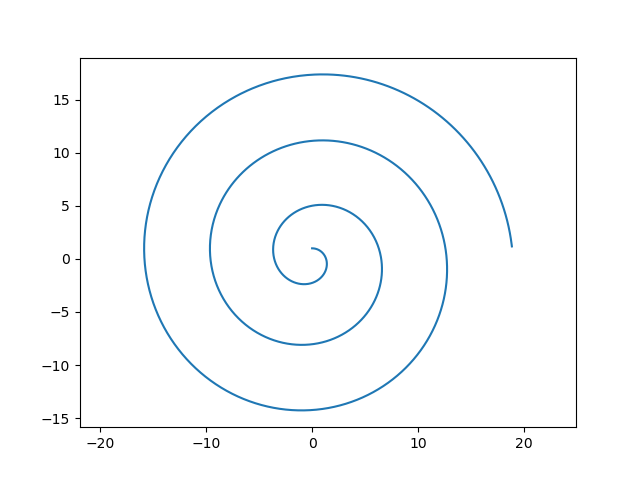
\includegraphics[width=\textwidth]{../figure/E_2_B160.png}
        \caption{Evenly Spaced Knots, $N=160$}
    \end{subfigure}
    \begin{subfigure}[b]{0.45\textwidth}
        \centering
        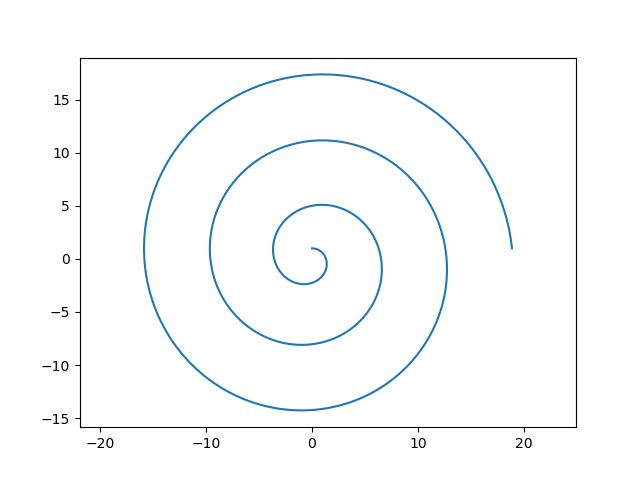
\includegraphics[width=\textwidth]{../figure/E_2_cum_B160.png}
        \caption{Cumulative Chordal Length, $N=160$}
    \end{subfigure}
\end{figure}

\subsection{III. Fit Three Dimension Curve}

For this question, I implement three ways to fit the curve
\begin{itemize}
    \item Directly fit, which may not on the surface of the ball. 
    \item Stereographic projection. 
    \item Spherical coordinates. 
\end{itemize}
Here just show the result of the last two methods. Here I use \textbf{Periodic Condition} to fit the curve.

For the Stereographic projection, we can have the following result
\begin{figure}[H]
    \centering
    \begin{subfigure}[b]{0.45\textwidth}
        \centering
        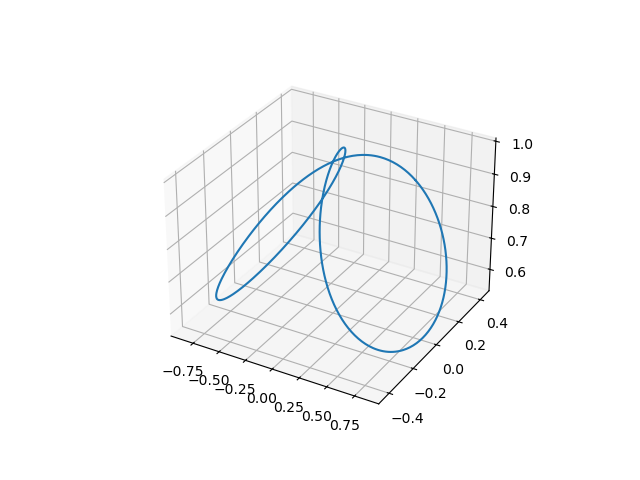
\includegraphics[width=\textwidth]{../figure/E_3_PPBallProj160.png}
        \caption{Evenly Spaced Knots, $N=160$}
    \end{subfigure}
    \begin{subfigure}[b]{0.45\textwidth}
        \centering
        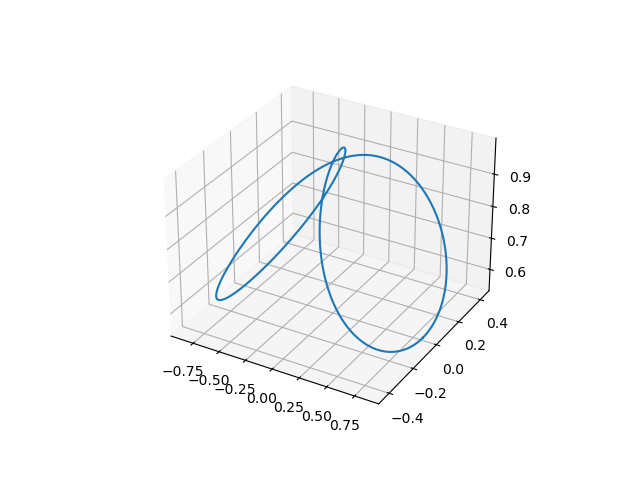
\includegraphics[width=\textwidth]{../figure/E_3_PPBallProj_cum160.png}
        \caption{Cumulative Chordal Length, $N=160$}
    \end{subfigure}
\end{figure}

For the Spherical coordinates, we can have the following result
\begin{figure}[H]
    \centering
    \begin{subfigure}[b]{0.45\textwidth}
        \centering
        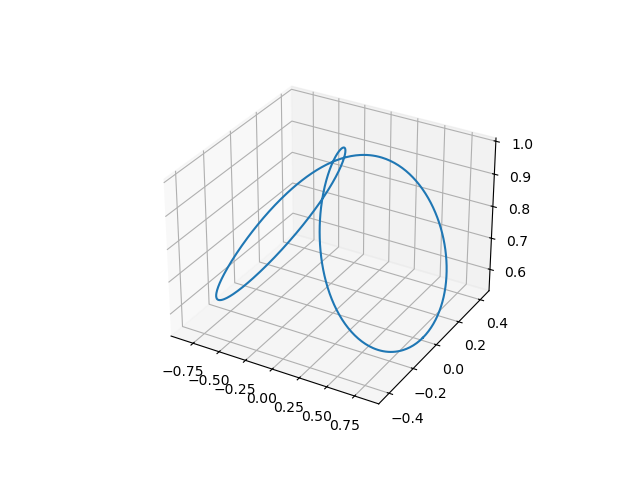
\includegraphics[width=\textwidth]{../figure/E_3_PPBall160.png}
        \caption{Evenly Spaced Knots, $N=160$}
    \end{subfigure}
    \begin{subfigure}[b]{0.45\textwidth}
        \centering
        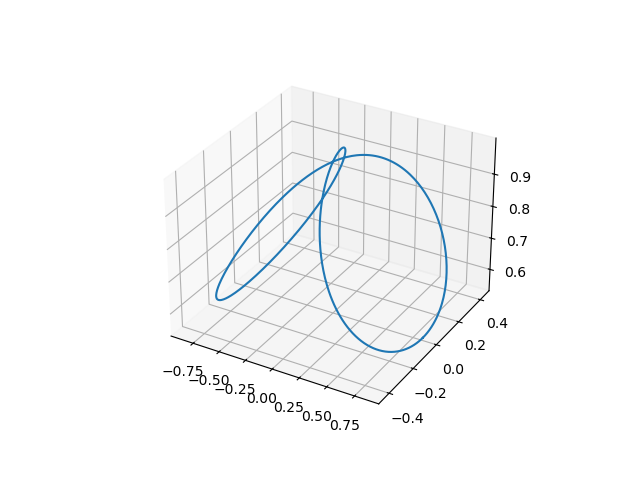
\includegraphics[width=\textwidth]{../figure/E_3_PPBall_cum160.png}
        \caption{Cumulative Chordal Length, $N=160$}
    \end{subfigure}
\end{figure}

The actual picture is as followings
\begin{figure}[H]
    \centering
    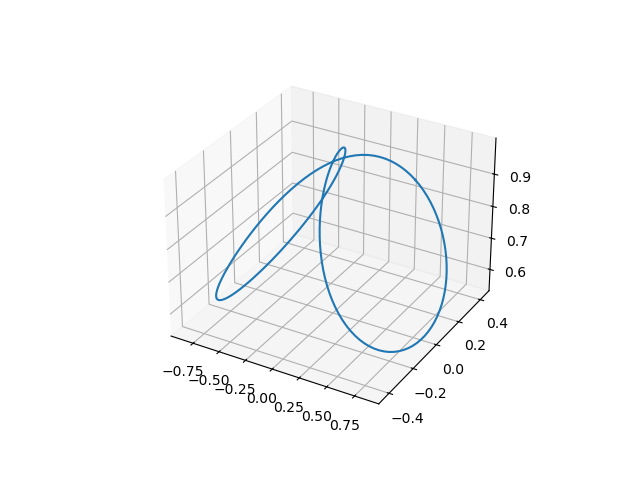
\includegraphics[width=0.5\textwidth]{../figure/EXACT160.png}
    \caption{Exact Curve}
\end{figure}

For the Cumulative Chordal Length, it's hard to determine which point is the actual point, for there is no condition, 
if we use the arc length, then we will just calculate the max error to determine which condition is better. 

Here just by observation, especially the heart curve, we may say that the cumulative chordal length is better.

\section{F. Truncated Power Functions}

The program is simple, just use the difinition of divided difference to calculate, and here are the results. 

\begin{figure}[H]
    \centering
    \begin{subfigure}[b]{0.5\textwidth}
        \centering
        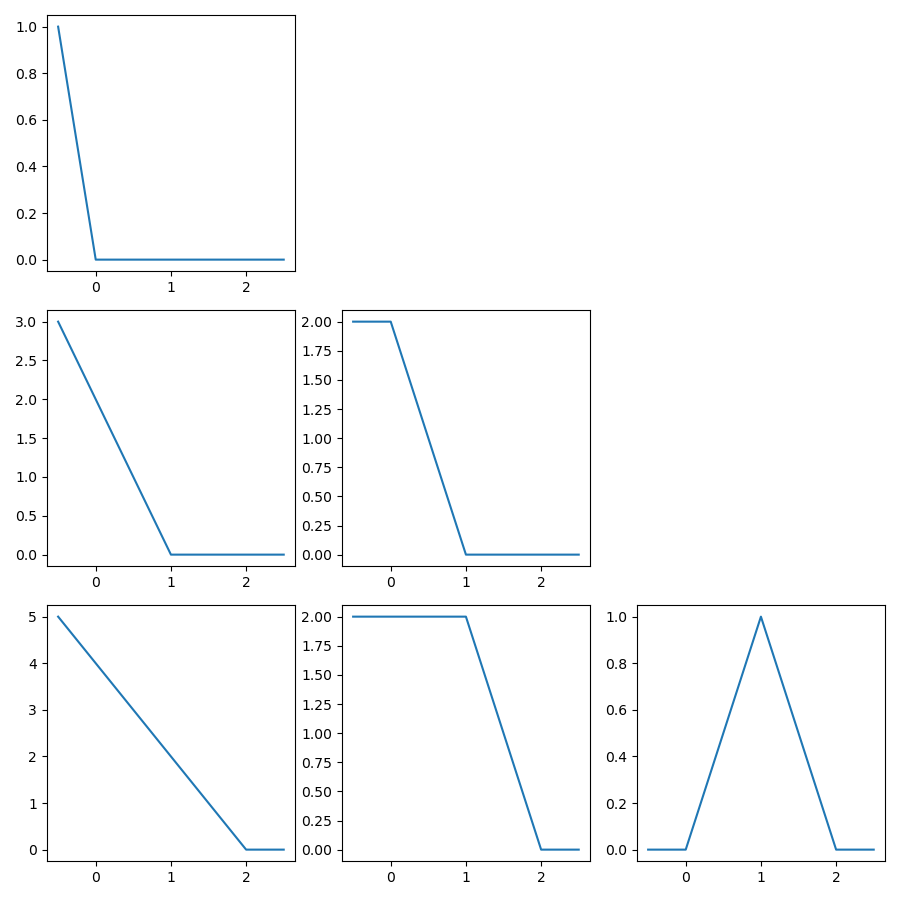
\includegraphics[width=\textwidth]{../figure/F_1.png}
        \caption{For $n=1$}
    \end{subfigure}
    \\
    \begin{subfigure}[b]{0.5\textwidth}
        \centering
        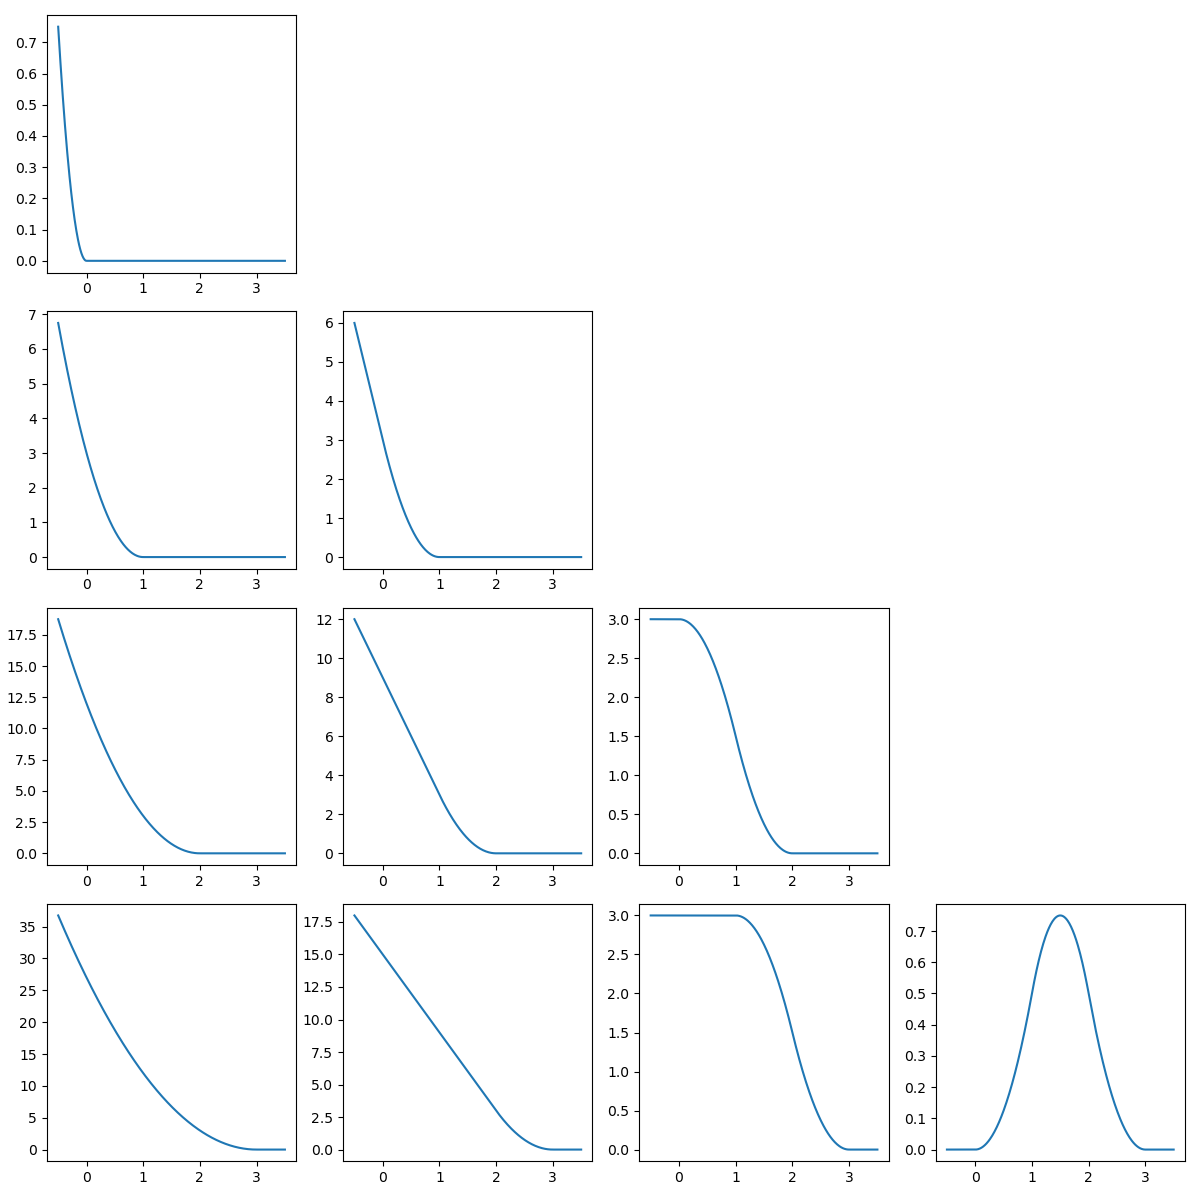
\includegraphics[width=\textwidth]{../figure/F_2.png}
        \caption{For $n=2$}
    \end{subfigure}
\end{figure}


\section{Appendix I. Verify that PP-form and B-form are equivalent}

In this section, we will design several experiments to verify that PP-form and B-form are equivalent under same knots and boundary condition. 
The result is obvious, because these conditions determine a unique polynomial in $\mathbb{S}_{n}^{n-1}$, which is proved in the book. The B-form is just 
the representation under a new basis, we can also use Bernstein polynomial as basis, which is not the focus of this section.

We choose the following functions to fit
\begin{itemize}
    \item $f(x) = 3+8x+4x^2+6x^3$
    \item $f(x) = \frac{1}{1 + e^{-x}}$
    \item $f(x) = \sin x + e^{-x}$
\end{itemize}

And here is the results, with $N = 10$.
\begin{figure}[H]
    \centering
    \begin{subfigure}[b]{0.45\textwidth}
        \centering
        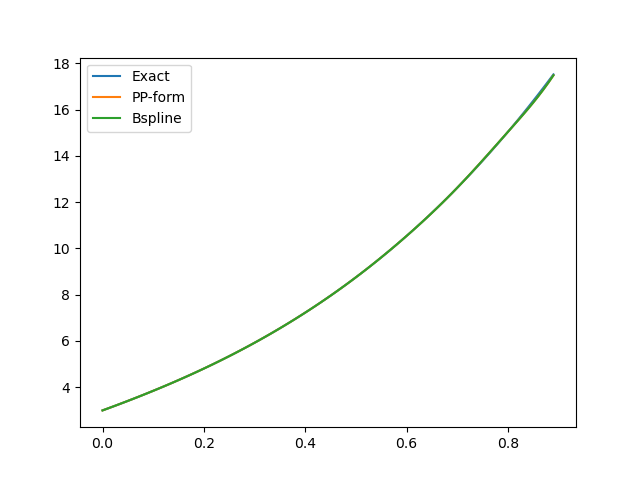
\includegraphics[width=\textwidth]{../figure/SplineTest1.png}
        \caption{$f(x) = 3+8x+4x^2+6x^3$}
    \end{subfigure}
    \begin{subfigure}[b]{0.45\textwidth}
        \centering
        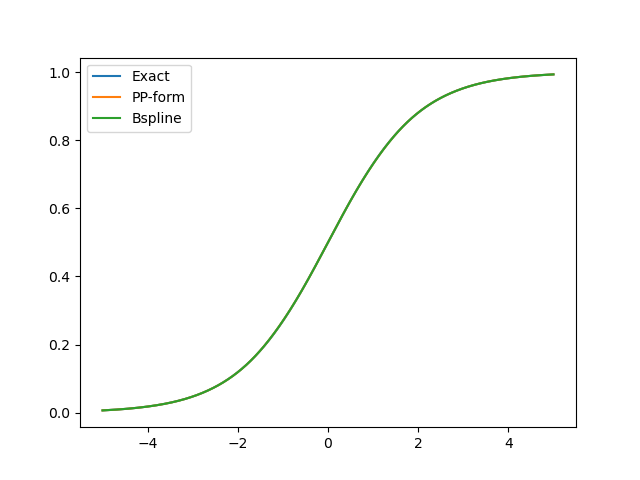
\includegraphics[width=\textwidth]{../figure/SplineTest2.png}
        \caption{$f(x) = \frac{1}{1 + e^{-x}}$}
    \end{subfigure}
    \\ 
    \begin{subfigure}[b]{0.45\textwidth}
        \centering
        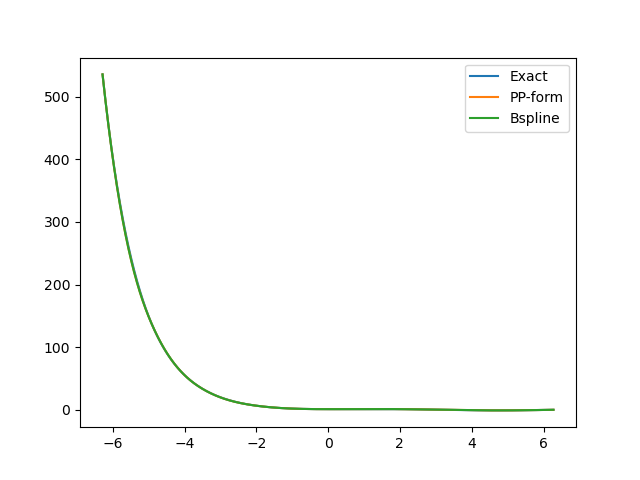
\includegraphics[width=\textwidth]{../figure/SplineTest3.png}
        \caption{$f(x) = \sin x + e^{-x}$}
    \end{subfigure}
    \caption{PP-form and B-form are equivalent}
    \label{FIG:APPENDIX1:1}
\end{figure}

Also, all results in Question E are also interpolated by both PP-form and B-form, and the results are the same, here just choose some of them to show, more results can be found in the \textbf{../figure/} folder.

\begin{figure}[H]
    \centering
    \begin{subfigure}[b]{0.45\textwidth}
        \centering
        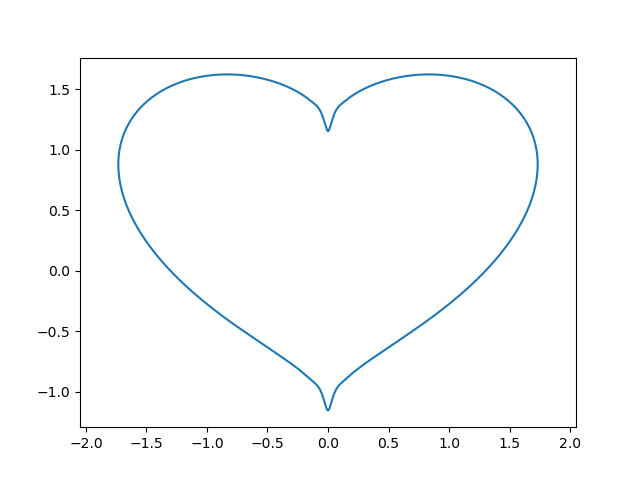
\includegraphics[width=\textwidth]{../figure/E_heart_cum_PP160.png}
        \caption{PP-form}
    \end{subfigure}
    \begin{subfigure}[b]{0.45\textwidth}
        \centering
        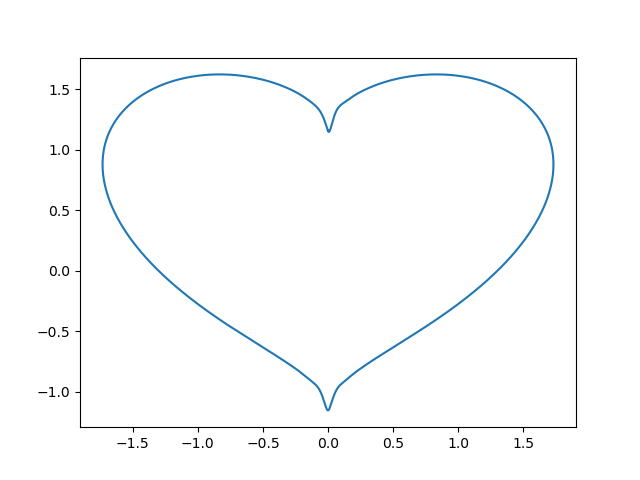
\includegraphics[width=\textwidth]{../figure/E_heart_cum_B160.png}
        \caption{Bspline}
    \end{subfigure}
    \\
    \begin{subfigure}[b]{0.45\textwidth}
        \centering
        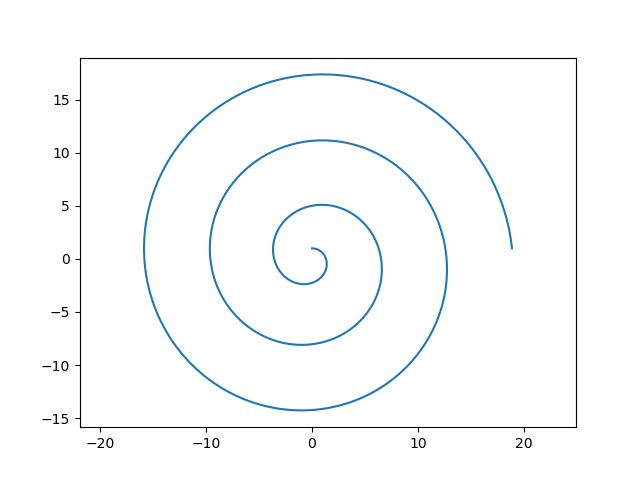
\includegraphics[width=\textwidth]{../figure/E_2_cum_PP160.png}
        \caption{PP-form}
    \end{subfigure}
    \begin{subfigure}[b]{0.45\textwidth}
        \centering
        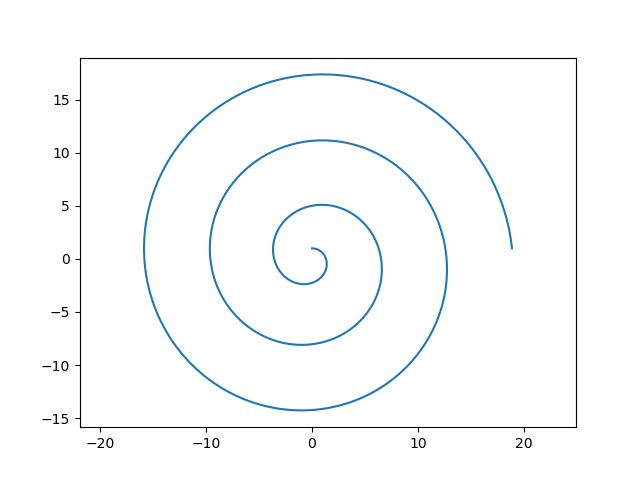
\includegraphics[width=\textwidth]{../figure/E_2_cum_B160.png}
        \caption{Bspline}
    \end{subfigure}
\end{figure}


\section{Appendix II. Error Estimation of Splines}

Under the same knots and boundary condition, the PP-form and B-form are equivalent,
so we just need to consider the PP-form.

For convenience, we assume $f \in C^{\infty}$

\subsection{$N=1$}
For the spline of oreder $1$, in each interval $[x_i, x_{i+1}]$, we know the spline is just the Lagrange interpolation,
so the error is 
\begin{equation}
    \abs{f(x) - s(x)} = \abs{\frac{f^{\prime \prime} (\xi)}{2} (x-x_i)(x-x_{i+1}) } \leq \frac{M}{8} h^2, M = \sup_{x \in [a,b]} \abs{f^{\prime \prime}(x)}, h = \max_{i} \abs{x_{i+1} - x_i}.
\end{equation}

Convergence rate is $2$.

\subsection{$N=2$}
For the spline of order $2$, this method may not be stable, take the following situation into consideration
\begin{equation}
    f(x) = \cos\qty(x), x \in [0, 100 \pi]. \quad
    t_i = i \pi, i = 0, 1, \cdots, 100.
\end{equation}
When given the first derivate at $0$, which is $0$, then by the relation
\begin{equation}
    m_i + m_{i+1} = 2 f[x_i, x_{i+1}],
\end{equation}
we can have $m_i = (-1)^i \frac{4 i}{\pi}$, then in the last interval we can have 
$m_{99} = -\frac{396}{\pi}$, then the polynomial is 
\begin{equation}
    p(x) = -1 - \frac{396}{\pi}(x-99 \pi) + \frac{398}{\pi^2}(x-99 \pi)^2.
\end{equation}
$h = \pi$ is the maximum interval, and all derivates of $f(x)$ is bounded, but as the number of knots increases, the error will increase.

So we can't find $C\in \mathbb{R}^{+}, j, N\in \mathbb{N}$, such that 
\begin{equation}
    \abs{f(x) - p(x)} \leq C h^j (\sum_{i=1}^{N} \sup_{x \in [a,b]} \abs{f^{(i)}(x)}), \forall x \in [a,b].
\end{equation}

\textbf{Similiar results may apply to all even order splines. Need to prove.}

\subsection{$N=3$}
For the spline of order $3$, we choose the \textbf{Complete Spline} to analysis. 

We first use Langrange interpolation to interpolate all second all derivates of $f(x)$, which is
\begin{equation}
    \hat{s}(x) = f^{\prime \prime}(x_i) + \frac{f^{\prime \prime} (x_{i+1}) - f^{\prime \prime}(x_i)}{x_{i+1}-x_i} (x-x_i), x \in [x_i, x_{i+1}].
\end{equation}

Then integrate $\hat{s}(x)$ twice, we can get a cubic spline $\tilde{s}(x)$, then we use complete cubic spline to interpolate 
$f - \tilde{s}$, which is $s - \tilde{s}$. Therefore, we can get the following error Estimation
\begin{equation}
    \abs{s^{\prime \prime}(x) - \tilde{s}^{\prime \prime}(x)} \leq 3 \max_{x \in [a,b]} \abs{f^{\prime \prime}(x) - \tilde{s}^{\prime \prime}(x)}.
\end{equation}

Finally we have 
\begin{equation}
    \abs{f^{\prime \prime} - s^{\prime \prime}} \leq \frac{1}{2} h^2 \max_{x \in [a,b]} \abs{f^{(4)}(x)}.
\end{equation}

For the first derivate, just integrate we can have
\begin{equation}
    f^{\prime}(x) - s^{\prime} (x) = \int_{x_i}^{x} f^{\prime \prime}(t) - s^{\prime \prime}(t) \, \mathrm{d}t.
\end{equation}
So we have 
\begin{equation}
    \abs{f^{\prime}(x) - s^{\prime} (x)} = (x - x_i) \abs{f^{\prime \prime}(\xi) - s^{\prime \prime}(\xi)} \leq \frac{1}{2} h^3 \max_{x \in [a,b]} \abs{f^{(4)}(x)}.
\end{equation}

Similiarly, we can have 
\begin{equation}
    \abs{f(x) - s(x)} = \frac{1}{2} h^4 \max_{x \in [a,b]} \abs{f^{(4)}(x)}.
\end{equation}

Actually, by the knowledge of Interpolation, we can have
\begin{equation}
    \abs{f(x) - s(x)} \leq \frac{1}{2} \abs{(x-x_i)(x-x_{i+1})} \max_{x \in [a,b]} \abs{f^{\prime \prime} (x) - s^{\prime \prime} (x)}
    \leq \frac{1}{16} h^4 \max_{x \in [a,b]} \abs{f^{(4)}(x)}.
\end{equation}

Also, we can implement some code to analysis this convergence rate, take a simple function 
\begin{equation}
    f(x) = \frac{1}{1 + 25 x^2}, x\in [-1, 1].
\end{equation}

If we have the relation 
\begin{equation}
    y = A h^k = A (\frac{2}{N-1})^k \Rightarrow \log y = C - k \log (N-1)
\end{equation}

And by LeastSquares, we can approx the rate of convergence as followings 
\begin{table}[H]
    \centering
    \begin{tabular}{|c|c|}
        \hline
        $N$ & Rate \\
        \hline
        1 & 1.95921 \\
        2 & 3.2433 \\
        3 & 4.21878 \\
        \hline
    \end{tabular}
\end{table}


\section{Appendix III. Error Estimation of Ball Fitting}

\subsection{I. Stereographic projection}

For the Stereographic projection, we choose $(x_0, y_0, z_0) \notin \gamma (t)$, then for $(x,y,z) \in \gamma (t)$, we have
\begin{equation}
    \tilde{x}(t) = \frac{z(t) x_0 - z_0 x(t)}{z(t)-z_0}, \tilde{y}(t) = \frac{z(t) y_0 - z_0 y(t)}{z(t)-z_0}.
\end{equation}

For simpicity, we assume $\gamma (t) \in C^{\infty}$, then we have
\begin{equation}
    \tilde{x}(t) \in C^{\infty}, \tilde{y}(t) \in C^{\infty}.
\end{equation}

Then, for the error estimation above, we take Cubic Spline as an example, we have 
\begin{equation}
    \begin{aligned}
        \abs{\tilde{x}(t) - s_x(t)} &\leq \frac{1}{16} h^4 \max_{t \in [a,b]} \abs{\tilde{x}^{(4)}(t)} = C_1 h^4, \\
        \abs{\tilde{y}(t) - s_y(t)} &\leq \frac{1}{16} h^4 \max_{t \in [a,b]} \abs{\tilde{y}^{(4)}(t)} = C_2 h^4.
    \end{aligned}
\end{equation}

Then, we push it back to the surface of the ball, we have
\begin{equation}
    \begin{aligned}
        l(t) &= \frac{2x_0 s_x(t)+2y_0 s_y(t) - 2 R^2}{R^2 - 2x_0 s_x(t) - 2y_0 s_y(t) + s_x(t)^2 + s_y(t)^2} \in C^{\infty}, \\
        \hat{x}(t) &= x_0 + l(t) (x_0 - s_x(t)), \\
        \hat{y}(t) &= y_0 + l(t) (y_0 - s_y(t)), \\
        \hat{z}(t) &= z_0 + l(t) (z_0 - z(t)).
    \end{aligned}
\end{equation}

We just need to determine 
\begin{equation}
    \abs{\hat{x}(t) - x(t)}, \quad \abs{\hat{y}(t) - y(t)}, \quad \abs{\hat{z}(t) - z(t)}.
\end{equation}

For simplicity, we write $x(t), y(t), z(t)$ as follows:
\begin{equation}
    \begin{aligned}
        l_1(t) &= \frac{2x_0 \tilde{x}(t)+2y_0 \tilde{x}(t) - 2 R^2}{R^2 - 2x_0 \tilde{x}(t) - 2y_0 \tilde{y}(t) + \tilde{x}(t)^2 + \tilde{y}(t)^2} \in C^{\infty}, \\
        x(t) &= x_0 + l_1(t) (x_0 - \tilde{x}(t)), \\
        y(t) &= y_0 + l_1(t) (y_0 - \tilde{y}(t)), \\
        z(t) &= z_0 + l_1(t) (z_0 - z(t)).
    \end{aligned}
\end{equation}

For $(x_0, y_0, z_0) \notin \gamma (t)$, we have $R^2 - 2x_0 \tilde{x}(t) - 2y_0 \tilde{y}(t) + \tilde{x}(t)^2 + \tilde{y}(t)^2 \ne 0$. 
Combine the error estimation above is enough. 


\subsection{II. Spherical coordinates}

Here we have 
\begin{equation}
    x(t) = r \sin \theta(t) \cos \varphi(t), \\
    y(t) = r \sin \theta(t) \sin \varphi(t), \\
    z(t) = r \cos \theta(t).
\end{equation}

So what we do is to interpolate $\theta(t)$ and $\varphi(t)$, also the same strategy as above, we can establish the error estimation.

\section{Appendix IV. Implement High Order Splines}

I have implemented the \textbf{PP-form} and \textbf{BSpline} with any order, and have tested them with the following functions. 
\begin{itemize}
    \item $f(x) = \sin\qty(x)$ 
    \item $f(x) = 3+8x+4x^2+6x^3$
    \item $f(x) = \frac{1}{1 + e^{-x}}$
    \item $f(x) = \sin\qty(x) + e^{-x}$
\end{itemize}

The results of this part has already put in Fig\ref{FIG:APPENDIX1:1}.

\section{Appendix V. Implement with Jsoncpp}
This part is not so difficult, just look at the file \path{../src/testjson.cc} to check the implementation.

\end{document}